% Written by Daina Chiba (daina.chiba@gmail.com).
% It was mostly copied from two poster style files:
% beamerthemeI6pd2.sty written by
%	 	Philippe Dreuw <dreuw@cs.rwth-aachen.de> and
% 		Thomas Deselaers <deselaers@cs.rwth-aachen.de>
% and beamerthemeconfposter.sty written by
%     Nathaniel Johnston (nathaniel@nathanieljohnston.com)
%		http://www.nathanieljohnston.com/2009/08/latex-poster-template/
% ---------------------------------------------------------------------------------------------------%
% Preamble
% ---------------------------------------------------------------------------------------------------%
\documentclass[final]{beamer}
\usepackage[orientation=landscape,size=custom,width=110,height=86,scale=1.2,debug]{beamerposter}
\mode<presentation>{\usetheme{RicePoster}}
\usepackage[english]{babel}
\usepackage[latin1]{inputenc}
\usepackage[T1]{fontenc}
\usepackage{amsmath,amsthm, amssymb, latexsym}

\usepackage{array,booktabs,tabularx}
\newcolumntype{Z}{>{\centering\arraybackslash}X} % centered tabularx columns


%   Begin Additional Packages
\usepackage{blindtext}
\usepackage{graphicx}
\usepackage{tikz}
%   End Additional Packages


% comment
\newcommand{\comment}[1]{}

\newlength{\columnheight}
\setlength{\columnheight}{80cm}
\newlength{\sepwid}
\newlength{\onecolwid}
\newlength{\twocolwid}
\newlength{\threecolwid}
\newlength{\restofpage}
\setlength{\sepwid}{0.024\paperwidth}
\setlength{\onecolwid}{0.24\paperwidth}
\setlength{\twocolwid}{0.4\paperwidth}
\setlength{\threecolwid}{0.19\paperwidth}
\setlength{\restofpage}{0.7\paperwidth}

% ---------------------------------------------------------------------------------------------------%
% Title, author, date, etc.
% ---------------------------------------------------------------------------------------------------%
\title{\huge deton8: Detector of Nuclei}
\author{Will LeVine \& Gabriel Vacaliuc}
\institute[Rice University]{Department of Computer Science, Rice University}
\date[Apr.2018]{April, 2018}
\def\conference{COMP540 Term Project: 2018 Data Science Bowl}
\def\yourEmail{wvl1@rice.edu,gv8@rice.edu}


% ---------------------------------------------------------------------------------------------------%
% Contents
% ---------------------------------------------------------------------------------------------------%
\begin{document}
\begin{frame}[t]

\begin{columns}[t]

\begin{column}{\onecolwid}

    \begin{block}{Introduction}
      \begin{itemize}
        \item Modern medicine generate lots of data that needs to be processed
        \item This often involves hand labeling data such as images
        \item It is desirable to automate this process
        \item One example is labeling microscopic nuclei in images
      \end{itemize}
    \end{block}

    \vskip3ex

    \begin{block}{Preprocessing \& Data Whitening}
        \begin{columns}[c]
            \column{.49\textwidth}
            \begin{itemize}
                \item since the input data is of a range of sizes, we reshape all
                    images to (256, 256)
                \item we negate all images with a white background so we can
                    assosciate brightness with nuclei
                \item since the color channels are highly correlated, we whiten
                    the data, resulting in greyscale images with reduced
                    modality effects
            \end{itemize}

            \column{.02\textwidth}

            \column{.49\textwidth}

            \begin{figure}
                \centering
                \caption{3D Plot of a sample of the training set.}
                \label{fig:correlated-features}
                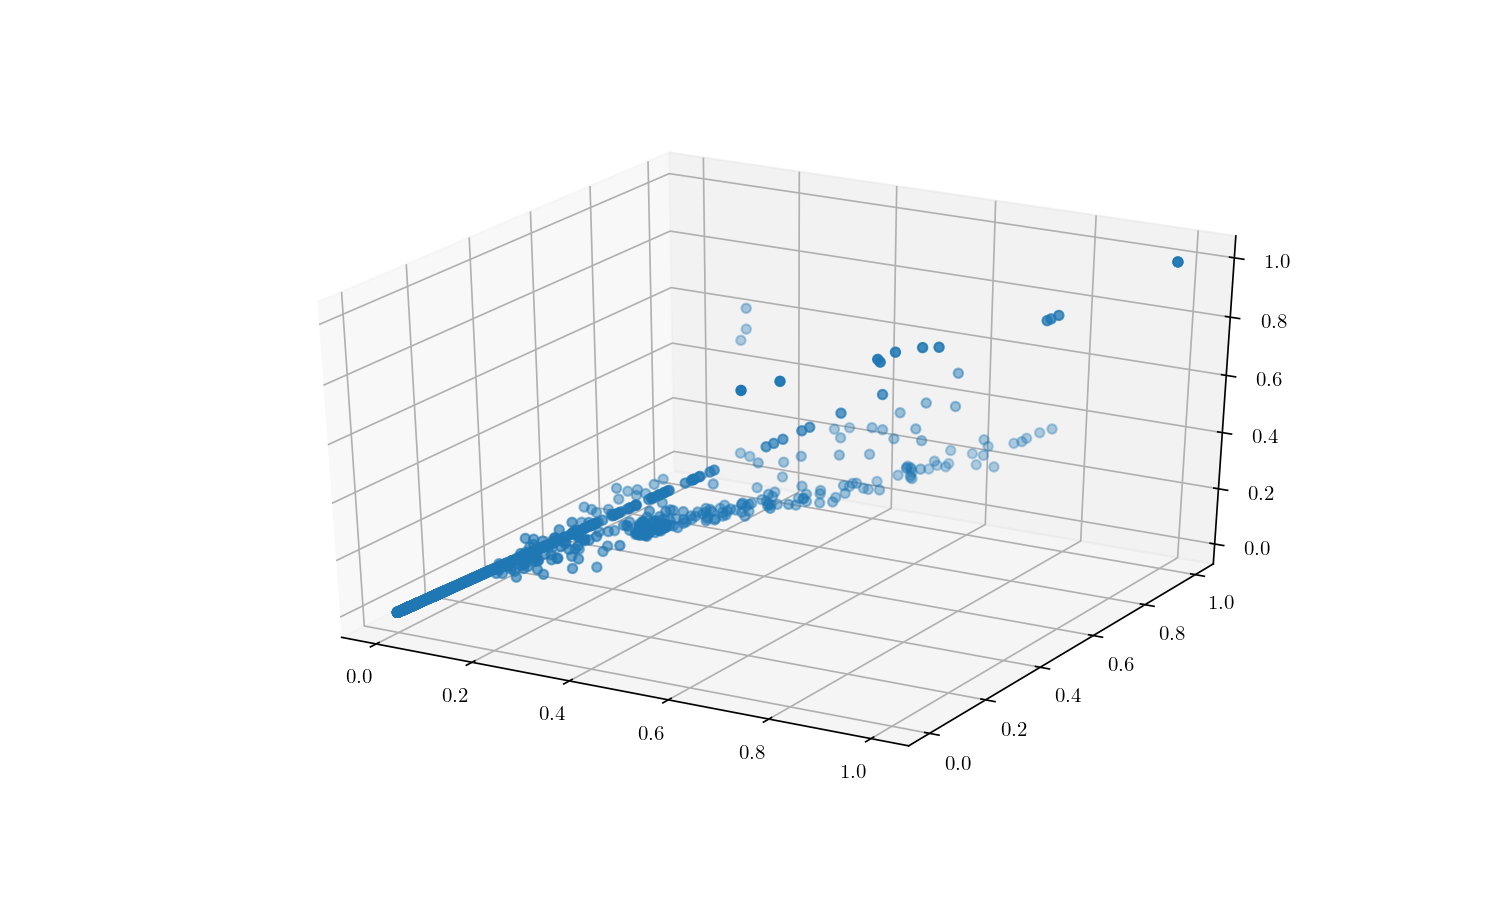
\includegraphics[width=\textwidth]{../paper/figs/correlated-features.png}
            \end{figure}
        \end{columns}

        \begin{figure}
            \centering
            \caption{Original Data.}
            \label{fig:correlated-features}
            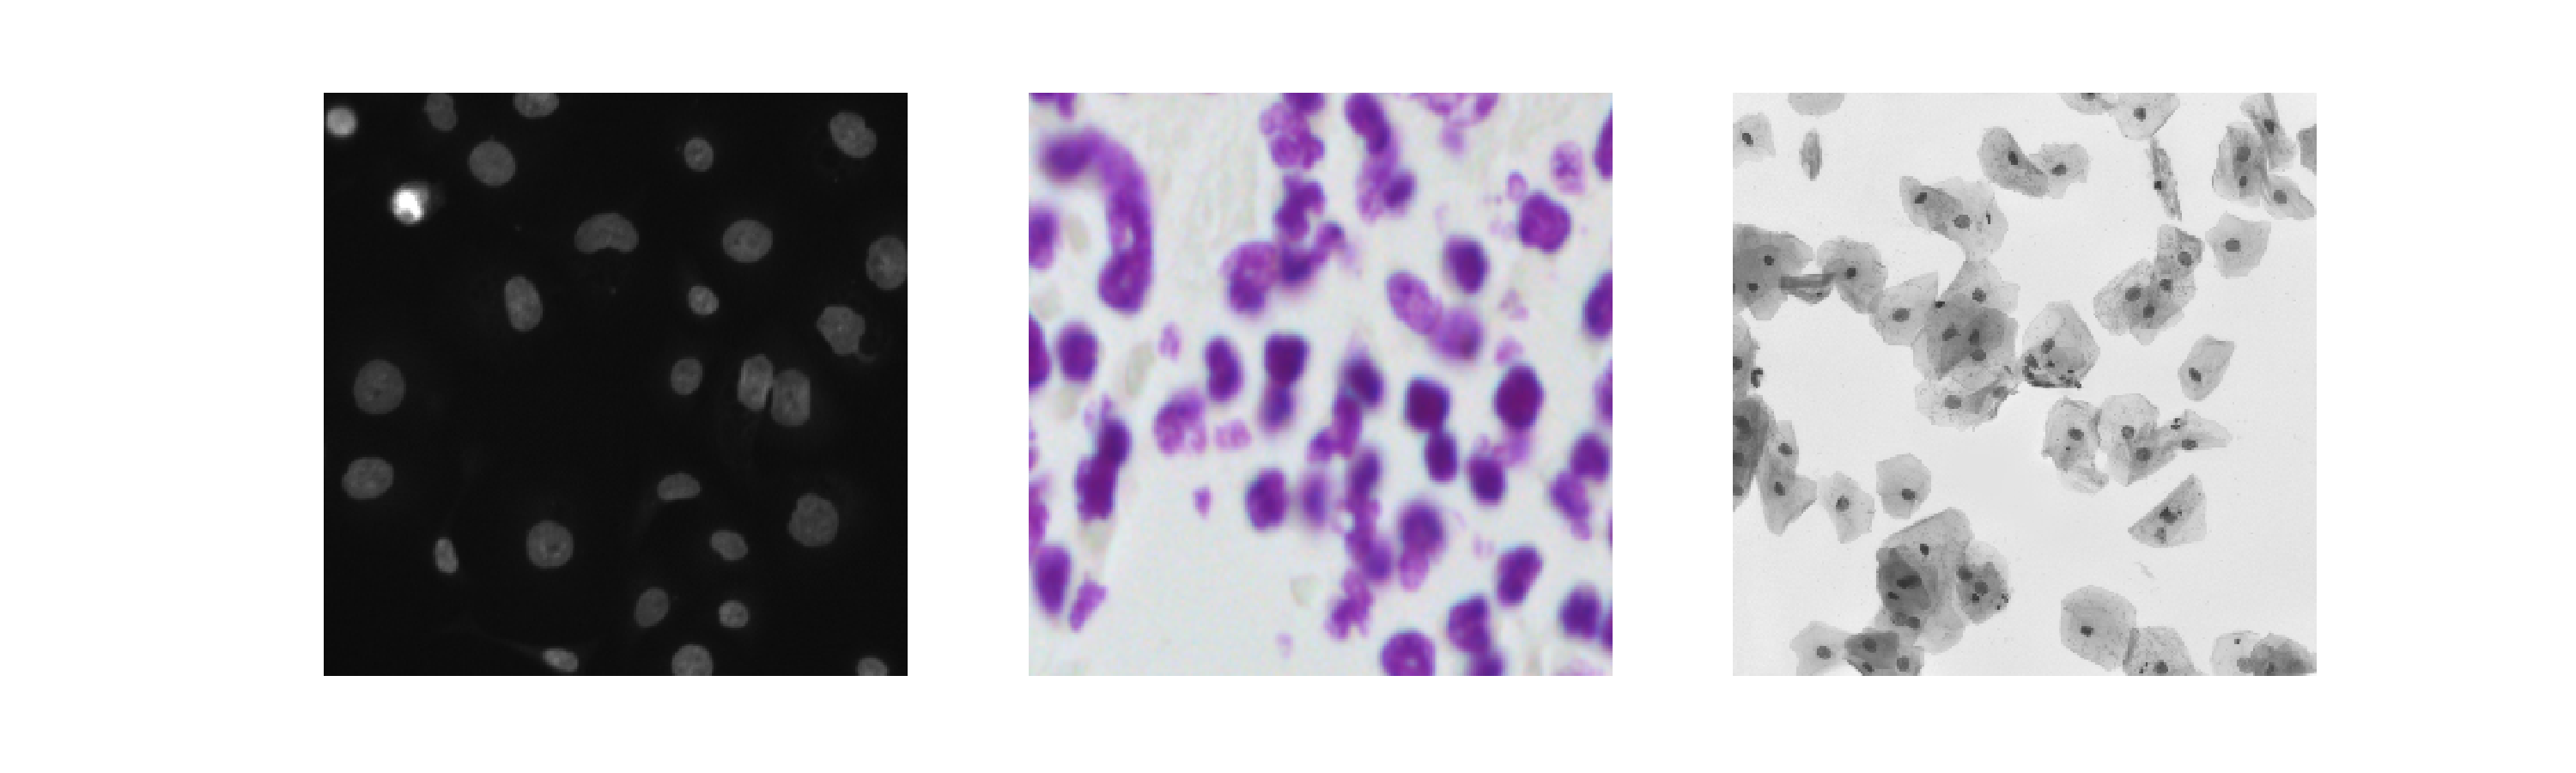
\includegraphics[width=\textwidth]{./figs/dsbowl18-imagegrid-1x3.png}
        \end{figure}

        \begin{figure}
            \centering
            \caption{Inverted and Whitened Data.}
            \label{fig:correlated-features}
            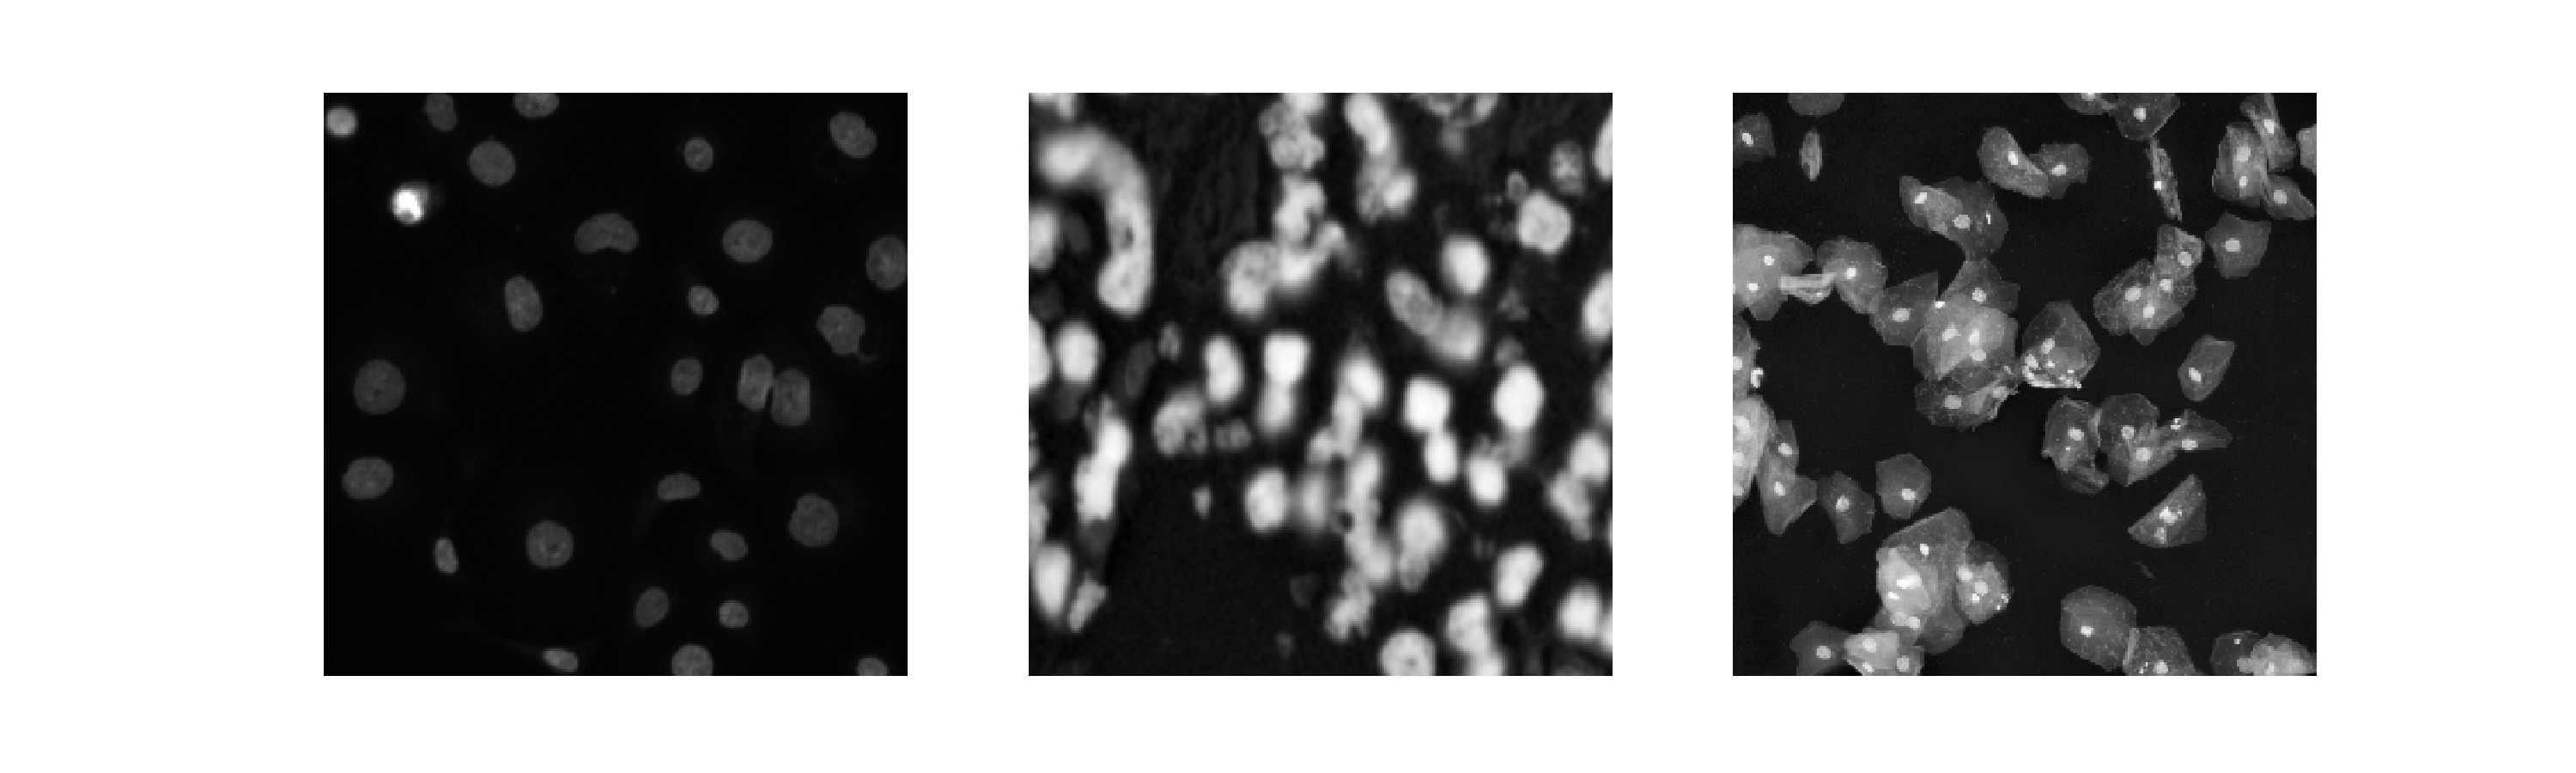
\includegraphics[width=\textwidth]{./figs/dsbowl18-imagegrid-1x3-whitened.png}
        \end{figure}

    \end{block}

    \vskip3ex

    \begin{block}{Hand Designed Features}
      \begin{itemize}
        \item Bilateral Filter: convolves image with weighted Gaussian kernel;
            denoises the image, while still preserving the edges
        \item 50/99 Image Rescaling: stretches pixel distribution; increases
            contrast between foreground and background
        \item Contrast Limited Adaptive Histogram Equalization: increases
            contrast locally; increases brightness of small nuclei
        \item Dilation: convolves image with uniform kernel; increases area of
            small nuclei
      \end{itemize}
    \end{block}

\end{column}

% -----------------------------------------------------------
% Start the second column
% -----------------------------------------------------------
\begin{column}{\restofpage}

    \begin{block}{Pipeline}
        \begin{tikzpicture}
        \node[inner sep=0pt] (raw) at (0,-13.5)
            {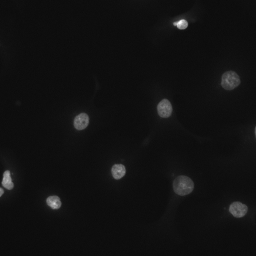
\includegraphics[width=8cm]{./figs/raw.png}};
        \node[inner sep=0pt] (raw lbl) at (0,-17.5)
            {Whitened Image};
        \node[inner sep=0pt] (bilateral) at (12,0)
            {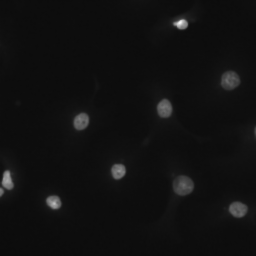
\includegraphics[width=8cm]{./figs/bilateral.png}};
        \node[inner sep=0pt] (bilateral lbl) at (12,-4)
            {Bilateral Filtering};
        \draw[->,line width=4pt] (raw.east) -- (bilateral.west);
        \node[inner sep=0pt] (rescale) at (12,-9)
            {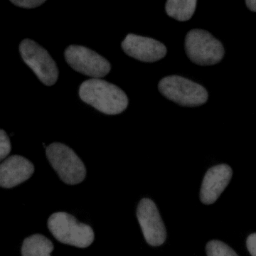
\includegraphics[width=8cm]{./figs/rescale.png}};
        \node[inner sep=0pt] (rescale lbl) at (12,-13)
            {Rescaling};
        \draw[->,line width=4pt] (raw.east) -- (rescale.west);
        \node[inner sep=0pt] (clahe) at (12,-18)
            {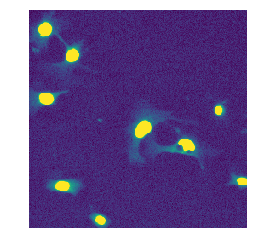
\includegraphics[width=8cm]{./figs/clahe.png}};
        \node[inner sep=0pt] (clahe lbl) at (12,-22)
            {CLAHE};
        \draw[->,line width=4pt] (raw.east) -- (clahe.west);
        \node[inner sep=0pt] (dilation) at (12,-27)
            {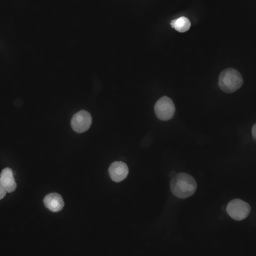
\includegraphics[width=8cm]{./figs/dilation.png}};
        \node[inner sep=0pt] (dilation lbl) at (12,-31)
            {Dilation};
        \draw[->,line width=4pt] (raw.east) -- (dilation.west);

        \node[inner sep=0pt] (sgd) at (24,-9)
            {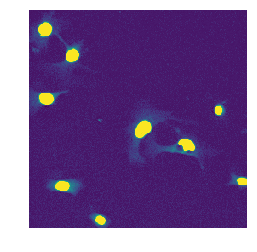
\includegraphics[width=8cm]{./figs/sgd.png}};
        \node[inner sep=0pt] (sgd lbl) at (24,-13)
            {SGD Output};
        \draw[-,line width=4pt] (rescale.east) -- (sgd.west);
        \draw[-,line width=4pt] (bilateral.east) -- (sgd.west);
        \draw[-,line width=4pt] (clahe.east) -- (sgd.west);
        \draw[-,line width=4pt] (dilation.east) -- (sgd.west);
        \node[inner sep=0pt] (pa) at (24,-18)
            {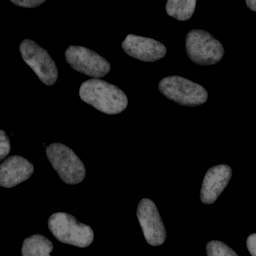
\includegraphics[width=8cm]{./figs/pa.png}};
        \node[inner sep=0pt] (pa lbl) at (24,-22)
            {PA Output};
        \draw[-,line width=4pt] (bilateral.east) -- (pa.west);
        \draw[-,line width=4pt] (rescale.east) -- (pa.west);
        \draw[-,line width=4pt] (clahe.east) -- (pa.west);
        \draw[-,line width=4pt] (dilation.east) -- (pa.west);

        \node[] (stack ptr) at (31.5, -13.5)
            {};
        \draw[-,line width=4pt] (raw.east) -- (stack ptr.west);
        \draw[-,line width=4pt] (sgd.east) -- (stack ptr.west);
        \draw[-,line width=4pt] (pa.east) -- (stack ptr.west);
        \node[inner sep=0pt] (raw stack) at (40,-10)
            {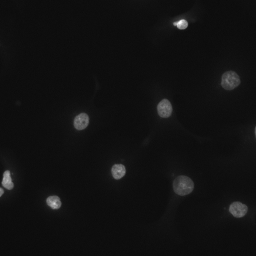
\includegraphics[width=8cm]{./figs/raw.png}};
        \node[inner sep=0pt] (bilateral stack) at (39,-12)
            {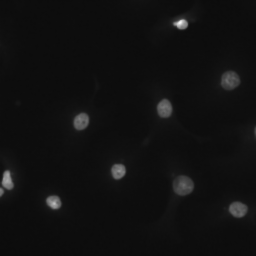
\includegraphics[width=8cm]{./figs/bilateral.png}};
        \node[inner sep=0pt] (rescale stack) at (38,-14)
            {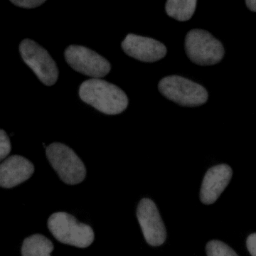
\includegraphics[width=8cm]{./figs/rescale.png}};
        \node[inner sep=0pt] (clahe stack) at (37,-16)
            {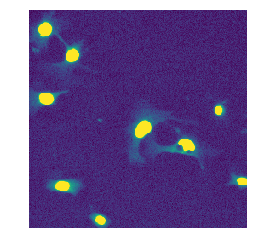
\includegraphics[width=8cm]{./figs/clahe.png}};
        \node[inner sep=0pt] (dilation stack) at (36,-18)
            {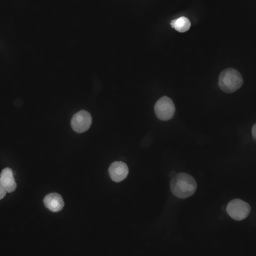
\includegraphics[width=8cm]{./figs/dilation.png}};
        \node[inner sep=0pt] (sgd stack) at (35,-20)
            {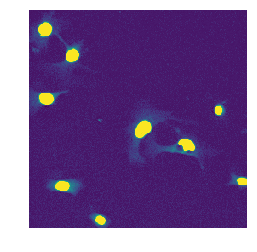
\includegraphics[width=8cm]{./figs/sgd.png}};
        \node[inner sep=0pt] (pa stack) at (34,-22)
            {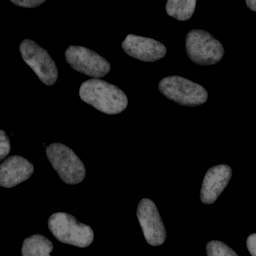
\includegraphics[width=8cm]{./figs/pa.png}};
        \node[inner sep=0pt] (stack) at (37,-26)
            {Stacked Features};

        
        \node[] (stack ptr right) at (44, -13.5)
            {};
        \node[inner sep=0pt] (unet output) at (50, -13.5)
            {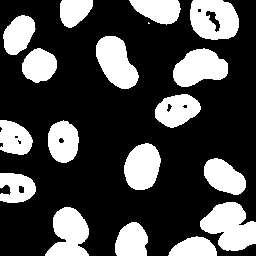
\includegraphics[width=8cm]{./figs/unet_output.png}};
        \node[inner sep=0pt] (unet lbl) at (50,-17.5)
            {UNet Output};
        \draw[->,line width=4pt] (stack ptr right.east) -- (unet output.west);
        \node[inner sep=0pt] (postprocessed) at (60, -13.5)
            {
\includegraphics[width=8cm]{./figs/postprocessed.png}};
        \node[inner sep=0pt] (postprocessed lbl) at (60,-17.5)
            {Postprocessed};
        \draw[->,line width=4pt] (unet output.east) -- (postprocessed.west);
        \node[inner sep=0pt] (segmentation) at (70, -13.5)
            {
\includegraphics[width=8cm]{./figs/seg.png}};
        \node[inner sep=0pt] (seg lbl) at (70,-17.5)
            {Watershed Segmentation};
        \draw[->,line width=4pt] (postprocessed.east) -- (segmentation.west); 

        \node[inner sep=0pt] (truth) at (70, -25)
            {
\includegraphics[width=8cm]{./figs/true_output.png}};
        \node[inner sep=0pt] (truth lbl) at (70,-29)
            {Ground Truth};
        \end{tikzpicture}
    \end{block}

    \begin{columns}[c]

        \column{0.33\textwidth}
        \begin{block}{Model Comparisons}
            \begin{tabular}{l|r}
                Model & Validation F1 Score \\ \hline
                PA-Regressor w/ Global Thresholding & 0.76 \\ \hline
                SGD-Regressor w/ Global Thresholding & 0.83 \\ \hline
                U-Net & 0.89
            \end{tabular}
        \end{block}

        \begin{block}{Score History}
          \begin{itemize}
            \item Kaggle Submissions: 40 sumissions entered uniformly
                throughout the past 3 months. No successful submissions other
                than provided sample submissions.
            \item Local implementation of Test Metric was run on Stage 1 Data,
                our pipeline received a score of a \textbf{0.316} on the
                competition metric.
            \item Git Commits: (176 Commits)
          \end{itemize}
              \begin{figure}
                  \centering
                  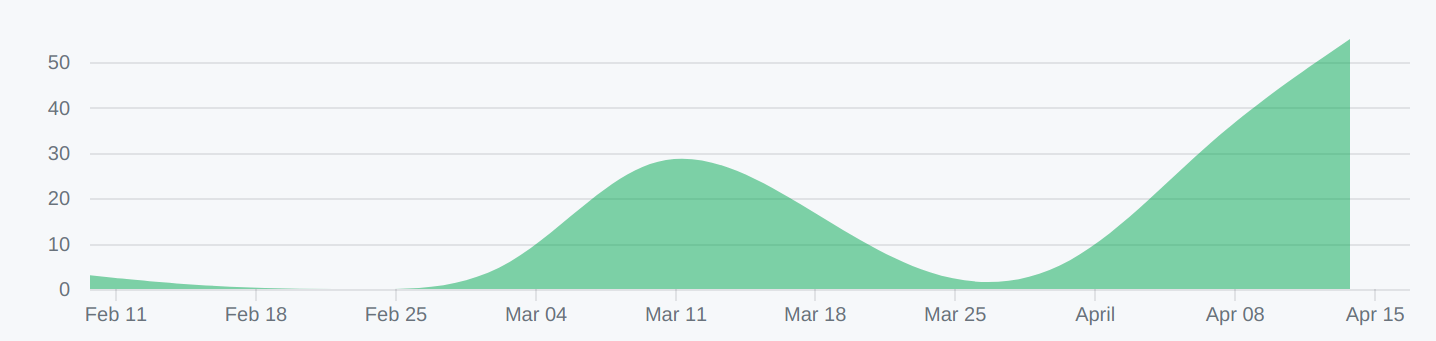
\includegraphics[width=\textwidth]{./figs/commit_graph.png}
                  \caption{Git Contributions}
              \end{figure}
        \end{block}

        \column{0.33\textwidth}
        \begin{block}{UNet} 
              \begin{figure}
                  \centering
                  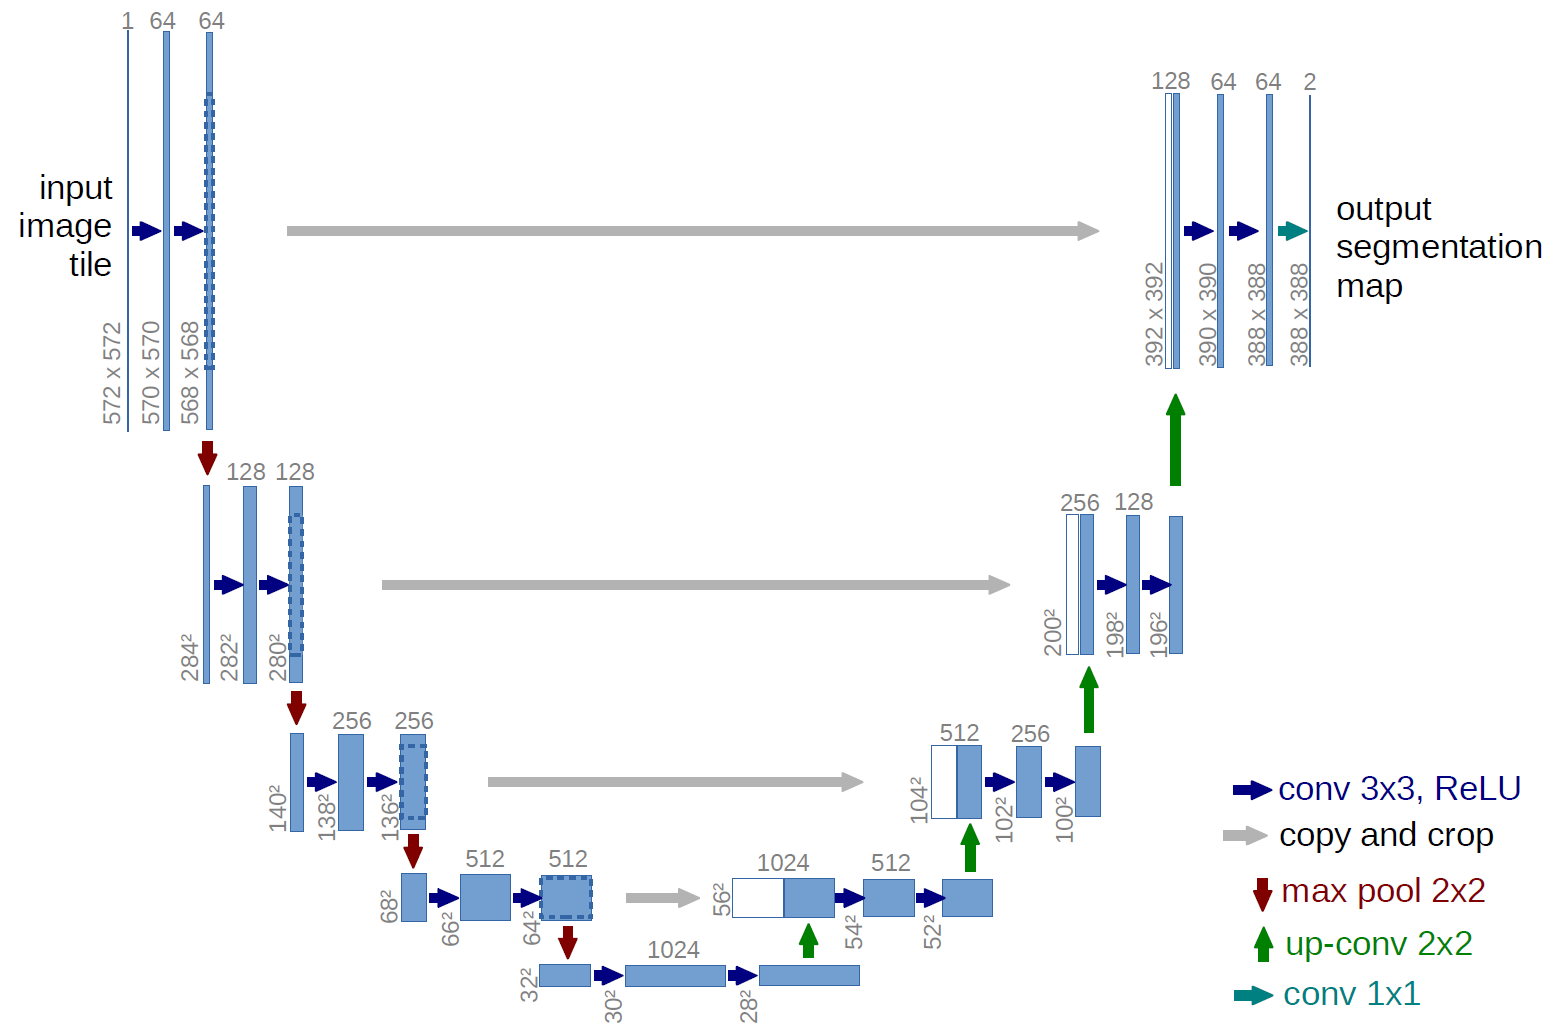
\includegraphics[width=.6\textwidth]{./figs/unet_architecture.png}
                  \caption{UNet Architecture}
              \end{figure}
              \begin{figure}
                  \centering
                  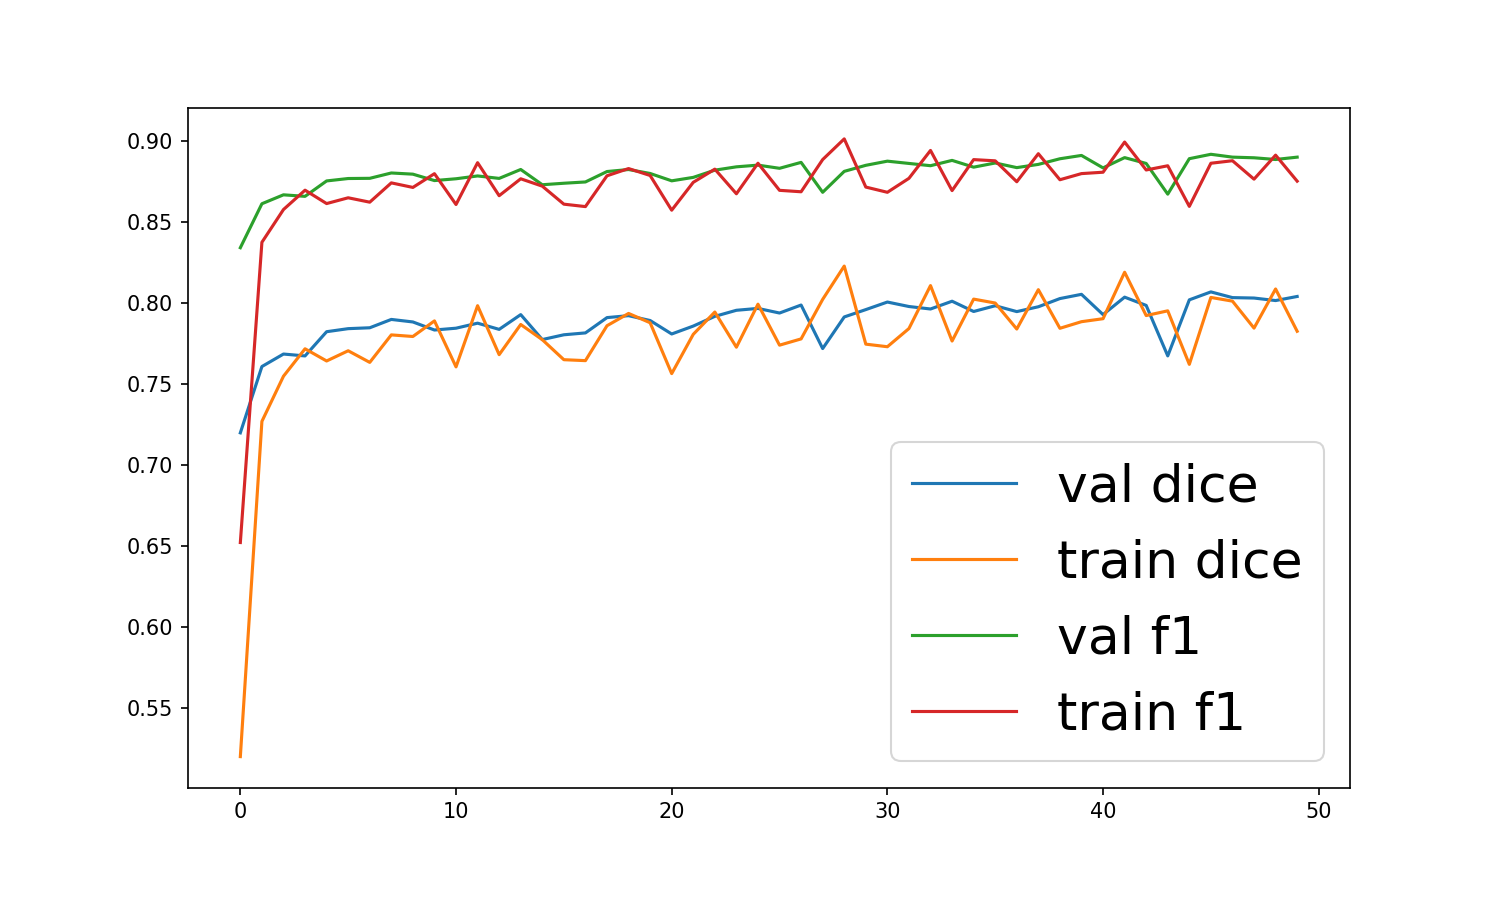
\includegraphics[width=.7\textwidth]{./figs/unet-score-history.png}
                  \caption{UNet Score History}
              \end{figure}
        \end{block}

        \column{0.33\textwidth}
        \begin{block}{Segmentation: \newline Non-Max Supression Watershed} 

            \centering
            Up close example of our segmentation process.

            \begin{tikzpicture}
                \node[inner sep=0pt] (dt) at (0, 0)
                    {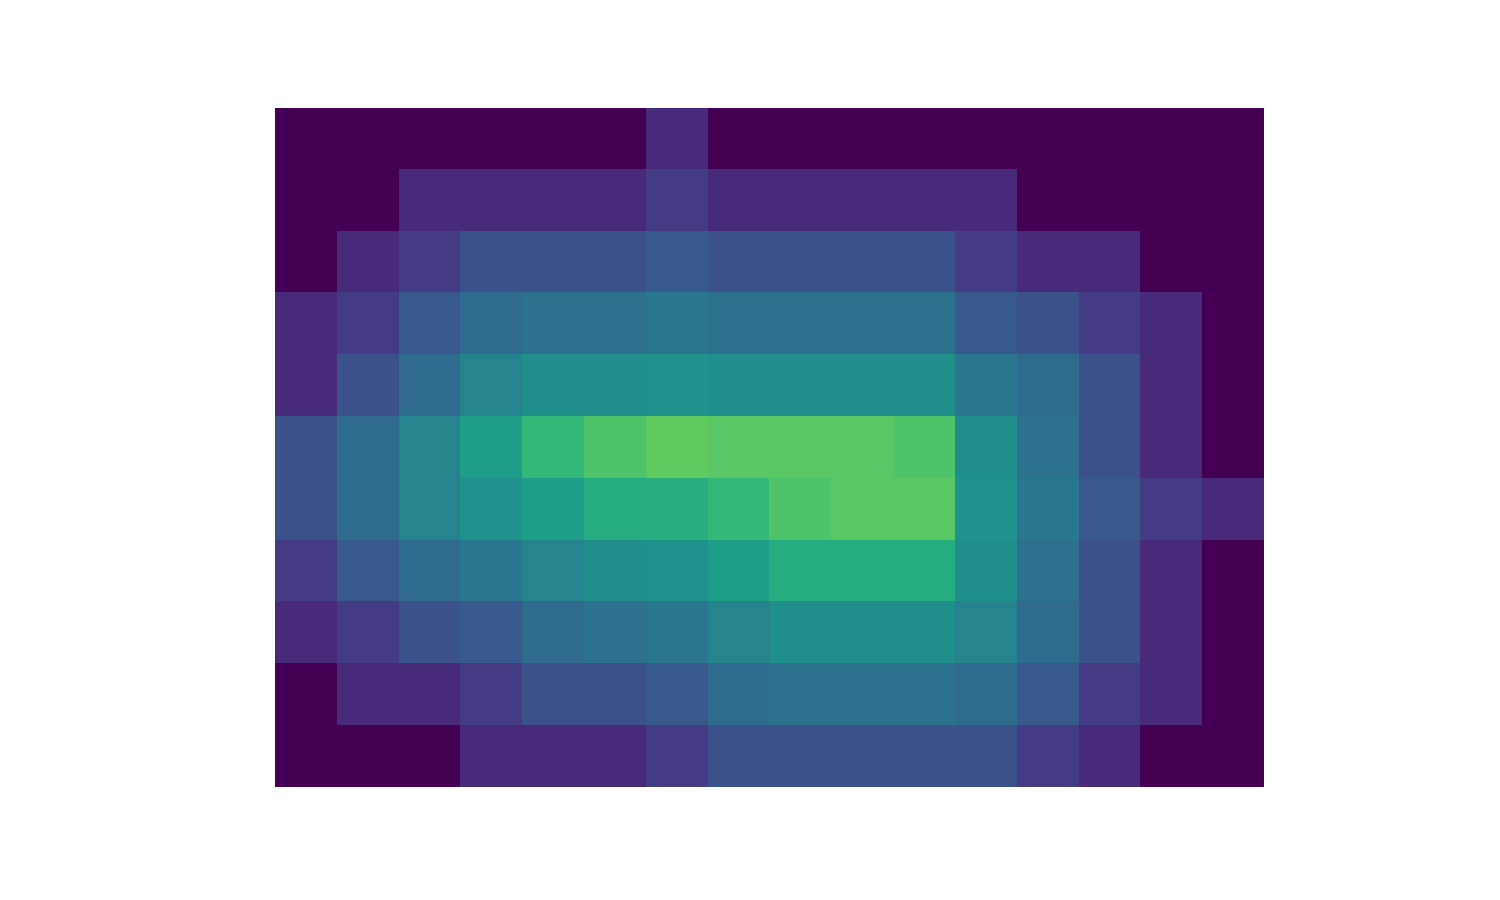
\includegraphics[width=8cm]{./figs/dt.png}};
                \node[inner sep=0pt] (dt lbl) at (0, -3)
                    {Distance Transform};

                \node[inner sep=0pt] (apeaks) at (15, 0)
                    {
\includegraphics[width=8cm]{./figs/avant_peaks.png}};
                \node[inner sep=0pt] (apeaks lbl) at (15, -3)
                    {Initial Local Maxes};

                \node[inner sep=0pt] (dpeaks) at (0, -10)
                    {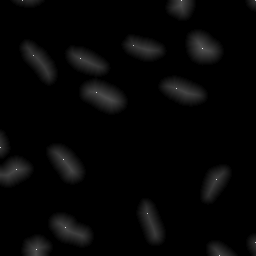
\includegraphics[width=8cm]{./figs/derriere_peaks.png}};
                \node[inner sep=0pt] (dpeaks lbl) at (0, -13)
                    {After Peak Filtering};

                \node[inner sep=0pt] (mask) at (15, -10)
                    {
\includegraphics[width=8cm]{./figs/seg_nuc.png}};
                \node[inner sep=0pt] (mask lbl) at (15, -13)
                    {Individual Nucleus Mask};

                \draw[->,line width=4pt] (dt.east) -- (apeaks.west); 
                \draw[->,line width=4pt] (apeaks.west) -- (dpeaks.north); 
                \draw[->,line width=4pt] (dpeaks.east) -- (mask.west); 
            \end{tikzpicture}
        \end{block}


    \end{columns}

\end{column}

\end{columns}

\end{frame}
\end{document}
